% !TEX root = ../../main.tex

% \section{Formal specification of a backend}
% \label{sec:formal-specification}
\section{System model}
\label{sec:system-model}

% In later sections, we will specify a generic model of transactions, with
% Multi-Version Concurrency Control (MVCC).
% The transaction model calls into a generic store model, with a versioned
% key-value interface.
% We refine the latter into three variants.

% consisting of query
% method \lookup{} and update methods \doUpdate{} and \doCommit{}.

Before tackling the bulk of the paper, this section states some
definitions and assumptions.
Table~\ref{tbl:notation} summarises our notations.

\subsection{Components of a store}

A store has a key-value interface, with versions identified by their
timestamps.
Keys, values, and timestamps are opaque types, denoted by the sets
$\Keytype$, $\Valuetype$ and \Timestamptype, ranged over by
meta-variables \akey, \aval and \atmstp{} respectively.

Timestamps are partially ordered by $\le$.
Timestamps are \emph{concurrent} if not mutually ordered:
$\atmstp[1] \concur \atmstp[2] \equaldef \atmstp[1] \not\le
\atmstp[2] \land \atmstp[2] \not\le \atmstp[1]$.

Two timestamps have a least upper bound $\max$ and a greatest lower
bound $\min$.
As a shorthand, $\max_{\atrset}(\asnpsht) \equaldef \max(
\Pi_{\asnpsht}(\atrset) )$ is the least-upper-bound of the \asnpsht{}
dimension in the set of tuples $\atrset$; and similarly for \acomstp{}.
We note $\atmstp[1] \geqq \atmstp[2] \equaldef \atmstp[1] \not<
\atmstp[2]$, read ``greater, equal, or concurrent.''
The notations $\min$ and $\leqq$ are defined symmetrically.

Classically, the timestamp type can be represented for instance by a
scalar integer (for strong-consistency) or a vector of integers, with
the classical definitions for $\le$ or $<$ \cite{alg:rep:738,
  alg:rep:738bis}.
In this case, we define $\max$ as follows:
  $\forall i: \max(\atmstp[1],\atmstp[2])[i] =
  \max(\atmstp[1][i],\atmstp[2][i])$; and similarly for $\min$.

\subsubsection{Effects}

A transaction updates a key by assigning a new value.
An update operation is called an \emph{effect} hereafter, noted
\aeffect{}.% 
%
\footnote{
%
  Our theory also supports operation-based CRDTs and more general
  effects \cite{syn:rep:sh143}, but for simplicity we keep this out of
  scope of this paper.
}
%
As an assignment masks any earlier assignments to the same key, earlier
ones can be ignored.
We assume that concurrent effects, if any, can be merged by an
appropriate \merge{} operator, which is is commutative, associative and
idempotent \cite{syn:rep:sh143, app:rep:1716}.
For instance, the popular last-writer-wins approach \merge{}s concurrent
assignments by putting a deterministic total order on their timestamps
and keeping only the highest one.

\subsubsection{Store}

A store, denoted $\astore \in \Storetype$, is a mapping from a
key-timestamp pair $(\akey,\atmstp)$ pair to an effect \aeffect{}.
An absent key-timestamp mapping is identified with \bottom{}.
Store API \cmdLookup{\astore{}}{\akey{}}{\atmstp{}} returns the effect
that store \astore{} associates with key \akey{} at time \atmstp{}.
For all practical purposes, this can be seen as a value.

Updating a key \akey{} under timestamp \atmstp{}
creates a new version tagged with \atmstp{}; a version is write-once.
A version is valid for the range of timestamps starting from its 
timestamp (excluded), until the next version, if any.

For example, suppose store \astore{} records assigns 27 to version 100 of
key \akey{} (assuming for the sake of example scalar timestamps).
Then, \cmdLookup{\astore{}}{\akey{}}{101} 
returns 27.
Furthermore, if there are no other versions between 100 and 110,
\cmdLookup{\astore{}}{\akey{}}{111} will also return 27.

% Note that an assignment masks any earlier versions of the same key.
% For all useful purposes, the key's versions may be truncated at its
% last assignment.

\subsection{Transactions}
\label{sec:timestamps-and-transactions}

An example transactional execution is illustrated in
Figure~\ref{fig:variants-and-composition}(a). 

A transaction is a sequence of effects.
Its reads come from a same \emph{snapshot} defined by a the
transaction's \emph{snapshot timestamp} (a.k.a.\ dependency timestamp)
noted \asnpsht{}.
The effects of a running transaction are not visible outside of it
(\emph{isolation}).
A transaction terminates in all-or-nothing manner: it either \emph{aborts},
and it makes no changes to the store; or it \emph{commits} with a
\emph{commit timestamp}.
In this case, its effects become visible in the store atomically,
labelled with the commit timestamp.
% Notation $\aeffect[\akey]^{\acomstp}$ refers to effect $\aeffect$
% updating key $\akey$ and committed with timestamp \acomstp{}.

As we define next, a transaction's snapshot \asnpsht{} has visibility of
an effect if and only if the latter's commit timestamp \acomstp{} is
strictly less than \asnpsht.

\subsection{Visibility}
\label{sec:visibility}

Effects are ordered by the \emph{visibility} relation $\aeffect[1]
\vis{} \aeffect[2]$ (read ``\aeffect[1] is visible to \aeffect[2]'')
defined as follows:
\begin{compactitem}
\item %[(Internal visibility INT)]
  $\aeffect \vis \aeffect'$ if both execute in the same transaction,
  and $\aeffect'$ executes before $\aeffect'$.
\item %[(External visibility EXT)]
  $\aeffect \vis \aeffect'$ if they belong to different transactions,
  \atrans{} and $\atrans'$ respectively, where $\atrans'$ can read from
  \atrans{}; formally, \atrans{} has committed, and $\atrans.\acomstp <
  \atrans'.\asnpsht$.
% \item % transitivity not necessary, because timestamp order is transitive
%   $\aeffect \vis \aeffect'$ if there exists $\aeffect''$ such
%   that $\aeffect \vis \aeffect'' \land \aeffect'' \vis \aeffect'$.
\end{compactitem}
%
Visibility is a partial order.%
%
\footnote{
%
  Note that even if timestamps form a total order (strong consistency),
  transactions might still be concurrent, for instance under Snapshot
  Isolation.
}
%
Committed effects that are not ordered are \emph{concurrent},
noted \concur{}.

\subsection{State of a store}
\label{sec:compose-effects}

Assume that at some point in time, the effects to key \akey{} are $ \{
\aeffect[i], \aeffect[j], \ldots{} \}$, ordered by \vis{}.
Then the expected state of a store maps \akey{} to $\max_{\vis}\{
\aeffect[i], \aeffect[j], \ldots{} \}$, defined as the result of
applying $\aeffect[i], \aeffect[j], \ldots{}$ in visibility order,
while \merge{}ing concurrent effects.

% Note that an uncommitted effect is \emph{not} considered concurrent to
% another transaction, since it is not visible outside of its transaction.

% \begin{figure}[tp]\small 
%   \begin{minipage}{1.0\columnwidth}
%     \centering
%     % -*-mode: latex; coding: utf-8-unix -*-
%
\[
\begin{array}{l}
    \aeffect[\akey] \compose \aeffect[\akey']' = \aeffect[\akey']' \compose \aeffect[\akey] = \\
      \ = \left\{
        \begin{array}{lll}
          \aeffect[\akey]    & \text{if}\ \aeffect[\akey']' = \bottom 		&  \text{(null effect)} \\
          \aeffect[\akey']'  & \text{if}\ \aeffect[\akey] = \bottom 		&  \text{(null effect)} \\
          \aeffect[\akey]    & \text{if}\ \aeffect[\akey] = \aeffect[\akey']' 	& \text{(idempotence)} \\
          \aeffect[\akey']' \circ \aeffect[\akey]
    %       = \aeffect[\akey] \circ \aeffect[\akey']' 
                             & \text{if}\ \akey \neq \akey' 			& \text{(independent keys)} \\

          \aeffect[\akey']' \circ \aeffect[\akey]
                             & \text{if}\ \aeffect[\akey] \vis \aeffect[\akey']' & \text{(apply in } \vis \text{ order)} \\
          \aeffect[\akey] \circ \aeffect[\akey']'
                             & \text{if}\ \aeffect[\akey']' \vis \aeffect[\akey] & \text{(apply in } \vis \text{ order)} \\
          \merge{}(\aeffect[\akey],\aeffect[\akey']')
     %     = \merge{}(\aeffect[\akey']',\aeffect[\akey])
                             & \text{if \merge{} def.}\
                               \land \aeffect[\akey] \concur \aeffect[\akey']'  & \text{(merge concurrent)} \\
 %         \ldots             & \text{and symmetrically} 			& \\
          \text{undefined}   & \text{otherwise}                                 & \text{(error)} \\

        \end{array}
        \right.
\end{array}
\]
\[
  \begin{array}[t]{rcl}
    (\aeffect'' \compose \aeffect') \compose \aeffect{}
    & = & \aeffect'' \compose (\aeffect' \compose \aeffect{}) \\
  \end{array}
\]

%% Local Variables:
%% coding: utf-8
%% mode: latex
%% eval: (auto-fill-mode -1)
%% ispell-local-dictionary: "en_GB"
%% mode: flyspell
%% TeX-master: "main" 
%% my-latex-bibfile: "~/svnbackup/bib/shapiro-bib-ext.bib"
%% End:

%   \end{minipage}
%   \caption{Effect composition}
%   \commentaire[SYSTOR]{Todo: remove effects, keep only assignments + merge.}
%   \label{fig:effect-composition}
% \end{figure}

\begin{figure*}[tp]
  \begin{minipage}{1.0\textwidth}
    \centering \small
    % -*-mode: latex; coding: utf-8-unix -*-
    \[
      \inferrule[\starttxnrule]
      {
        \atrans \notin \Pi_{\atrans}(\atrseta \cup \atrsetc \cup \atrsetr)
        \\
        % \consistencyBegin{\astore}{\atrseta}{\atrsetc}{\atrsetr\ }
        % \\
        \\
        % Visibility clause: must not depend on a transaction that will
        % commit in the future
        \forall t \in \Pi_{\acomstp}(\atrsetr): t \not< \asnpsht
        \\
        % \atrsetr' = \atrsetr\ \cup\ \{(\atrans, \asnpsht, \empeffbuf, \emptyset, +\infty)\}
      }
      {
        \astate \xrightarrow[\atrans]{\cmdBeTr}
        \bstate{\afield[\astore]}{\atrseta}{\atrsetc}{\atrsetr'}
      }
  \]

  \[
    \inferrule[\initkeyrule]
    {
      \atrsetr = \atrsetr'' \cup \{(\atrans, \asnpsht, \areadset, \adirtyset, \astatebuf, +\infty)\}
      \\
      \akey \notin {\areadset}
      \\
      \cmdLookup{\astore}{\akey}{\asnpsht} = \aeffect
      \\
      \areadset' = \areadset \union \{ \akey \}
      \\
      \astatebuf' = \astatebuf [\akey \leftarrow \aeffect ]
      \\
      \atrsetr' = \atrsetr''
      \cup \{(\atrans, \asnpsht, \areadset', \adirtyset, \astatebuf', +\infty)\}
    }
    {
      \astate \xrightarrow[\atrans]{}
      \bstate{\afield[\astore]}{\atrseta}{\atrsetc}{\atrsetr'}
    }
  \]

  % \commentaire[Marc 2023-02-08]{Somewhere, add the constraint that
  %   \aeffect{} above must resolve to a \Valuetype{} in the top-level composed
  %   store.}
  
  \[
    \inferrule[\readrule]
    {
      \atrsetr = \atrsetr'' \cup \{(\atrans, \asnpsht, \areadset, \adirtyset, \astatebuf, +\infty)\}
      \\
      \akey \in {\areadset}
      \\
      \astatebuf(\akey) = \aval
    }
    {
      \astate \xrightarrow[\atrans]{\cmdRead{\akey} \rightarrow \{\aval\}}
      \astate
    }
  \]

  \[
    \inferrule[\updaterule]
    {
      \atrsetr = \atrsetr''
        \cup \{(\atrans, \asnpsht, \areadset, \adirtyset, \astatebuf, +\infty)\}
      \\
        \akey \in \areadset
      \\
        \astore' = \cmdDoUpdate{\astore}{\atrans}{\akey}{\aeffect}
        \\
        \adirtyset' = \adirtyset{} \union \akey
        \\
        \astatebuf' = \astatebuf{}[\akey \leftarrow \aeffect{}
        (\astatebuf(k))]
        \\
      \atrsetr' = \atrsetr''
        \cup \{(\atrans, \asnpsht, \areadset,
               \adirtyset',
               \astatebuf',
               +\infty)\}
    }
    {
      \astate \xrightarrow[\atrans]{\cmdUpdate{\atrans}{\akey}{\aeffect}}
      \bstate[\astore']{\afield[\astore]}{\atrseta}{\atrsetc}{\atrsetr'}
    }
  \]

  \[
    \inferrule[\abortrule]
    {
      \atrsetr = \atrsetr'
      \cup \{(\atrans, \asnpsht, \areadset, \adirtyset, \astatebuf, +\infty)\}
      \\
      \atrseta' = \atrseta
      \cup \{(\atrans, \asnpsht, \areadset, \adirtyset, \astatebuf, +\infty)\}
    }
    {
      \astate \xrightarrow[\atrans]{\cmdAbort}
      \bstate{\afield[\astore]}{\atrseta'}{\atrsetc}{\atrsetr'}
    }
  \]  


  \[
    \inferrule[\commitrule]
    {
      \atrsetr = \atrsetr'
      \cup \{(\atrans, \asnpsht, \areadset, \adirtyset, \astatebuf, +\infty)\}
      \\
      \acomstp \notin \Pi_{\acomstp}(\atrsetc)
      \\
      \asnpsht \le \acomstp
      \\
      % Visibility clause: must not commit after a dependent transaction
      % started = *Crucial For Correctness*!!!
      % Moved to BEGIN_TRANSACTION
      % \forall \atmstp \in \Pi_{\asnpsht}(\atrsetc \union \atrsetr):
      %     \acomstp \not< \atmstp %%% CRUCIAL
      % \\
      % \CCCommit[]{\astore}{\atrsetc}{\acomstp}{\areadset}{\adirtyset}{\astatebuf}{\atrsetc}
      % \\
      \astore' = \cmdDoCommit{\astore}{\atrans}{\areadset}{\adirtyset}{\astatebuf}{\acomstp}
      \\
      \atrsetc' = \atrsetc
      \cup \{(\atrans, \asnpsht, \areadset, \adirtyset, \astatebuf, \acomstp)\}
    }
    {
      \astate \xrightarrow[\atrans]{\cmdCommit{\acomstp}}
      \bstate[\astore']{\afield[\astore]}{\atrseta}{\atrsetc'}{\atrsetr'}
    }
  \]


%% Local Variables:
%% mode: latex
%% coding: utf-8
%% ispell-local-dictionary: "en_GB"
%% mode: flyspell
%% TeX-master: "main" 
%% my-latex-bibfile: "~/svnbackup/bib/shapiro-bib-ext.bib"
%% End:

  \end{minipage}
\caption{Operational Semantics of Transactions}
  \label{fig:transaction-semantics}
\end{figure*}
\begin{figure}[tp]
  \centering \small
  % -*-mode: latex; coding: utf-8-unix -*-

\[
  \begin{array}{rcl}
    \lookup{}   & : & \Storetype
                      \times \Keytype
                      \times \Timestamptype 
                      \rightarrow \Effecttype_{\bottom}\\
    \doUpdate{} & : & \Storetype
                      \times \TransactionIDtype
                      \times \Keytype
                      \times \Effecttype 
                      \rightarrow \Storetype \\
    \doCommit{} & : & \Storetype
                      \times \TransactionIDtype
                      \times \mathcal{P}(\Keytype)
                      \times \mathcal{P}(\Keytype)
                      \times \Statebuftype
                      \times \Timestamptype
                      \rightarrow \Storetype\\
  \end{array}
\]


%% Local Variables:
%% mode: latex
%% coding: utf-8
%% ispell-local-dictionary: "en_GB"
%% mode: flyspell
%% TeX-master: "main" 
%% my-latex-bibfile: "~/svnbackup/bib/shapiro-bib-ext.bib"
%% End:

  \caption{Store interface}
  \label{fig:store-interface}
\end{figure}

\section{A formal model, from a systems perspective}
\label{sec:transaction-framework}

In this section, we study a formal model of transactions and store
operations, focusing on what they say from a systems perspective.

\subsection{Semantics of transactions}
\label{sec:formal-semantics}

Figure~\ref{fig:transaction-semantics} presents the semantics of
transactions.
The specification is fully formal and unambiguous: we find it invaluable
to reason about the system, and it is easily translated to the language
of a proof tool such as Coq.
Most interestingly, it can be read as pseudocode, as we explain now.

\subsubsection{Informal presentation}

The semantics are written as a set of rules.
A rule consists of a set of \emph{premises} above a long horizontal
line, and a \emph{conclusion} below.
A premise is a logical predicate, specifying expected pre-state
(unprimed variables) or post-state (primed variables).
If the premises are satisfied, the state-change transition described by
the conclusion can take place.
A label on the transition arrow under the line represents a client API
call.
Thus a rule can be seen as terse pseudocode for the computation to be
carried out by the API.

To explain the syntax, consider for example rule \starttxnrule{}.
The conclusion describes the transition made by API \cmdBeTr[\asnpsht]
from pre-state \astate{} on the left
of the arrow $\xrightarrow[\atrans]{\cmdBeTr}$, to post-state
$\bstate{\afield[\astore]}{\atrseta}{\atrsetc}{\atrsetr'}$ on the right.
The premise is a set of logical conditions; one that uses only
non-primed variables is a pre-condition on the prestate; if it contains
a primed variable, it is a post-condition that constrains the
post-state.
Note that in the right-hand side of this conclusion, only \atrsetr{} is
primed, indicating that the other elements of the state do not change.
Such a transition is atomic, i.e., there are no intermediate states from
a semantic perspective; any intermediate states in the implementation
must not be observable.

The system is defined as a tuple $\astate$ consisting of a store, its
field, and the sets of aborted, committed, and running transactions'
descriptors.
Recall from Table~\ref{tbl:notation} that a transaction descriptor is a
tuple composed of its identifier \atrans, its \emph{dependency
  timestamp} \asnpsht, its \emph{read set} \areadset, its \emph{dirty set}
\adirtyset, its \emph{state buffer} \astatebuf, and its \emph{commit
  timestamp} \acomstp.
We will ignore \afield[\astore{}]{} until
Section~\ref{sec:composed-store-variant}.

The rules are parameterised by commands \lookup{}, \doUpdate{} and
\doCommit{} (Figure~\ref{fig:store-interface}), which are specialised
for each specific store variant, as detailed later.
% : the map-based variant in
% Section~\ref{sec:map-store-variant}, the journal-based variant in
% Section~\ref{sec:journal-store-variant}, and composition variant in
% Section~\ref{sec:composed-store-variant}.

% We now describe the rules in turn, then identify the implementation
% issues that they raise.

% The rules are also parameterised for consistency model, via
% preconditions \cmbegin{} and \cmcommit.
% In our baseline TCC consistency model, they are empty (i.e., true).
% In future work, they will be adapted to support stronger consistency
% models.

\subsubsection{Transaction begin}

\starttxnrule{} describes how API $\cmdBeTr$ begins a new
transaction with dependency timestamp \asnpsht{}.
The first premise chooses a fresh transaction identifier
\atrans{}.
% (it is not in the union of transaction
% descriptors, $\atrseta \cup \atrsetc \cup \atrsetr$, projected by
% $\Pi_{\atrans}$ along the $\atrans$ dimension).
The last premise adds a transaction descriptor to the set of running
transactions.

The snapshot of the new transaction is timestamped by \asnpsht, passed
as an argument.
Remember that a snapshot includes all transactions that committed with
a strictly lesser commit timestamp.
The \emph{visibility} premise $\forall t \in \Pi_{\acomstp}(\atrsetr): t
\not< \asnpsht$ states that the new transaction may not depend on some
transaction that is not yet terminated.
Suppose this premise was not present: then this transaction might attempt
to read a value that has not yet been written or will be aborted.
We discuss the synchronisation required for enforcing it in
Section~\ref{sec:enforce-visibility}.

As the transition is labeled by \atrans{}, multiple instances of
\starttxnrule{} are mutually independent and might execute in parallel,
as long as each such transition appears atomic.

\subsubsection{Reads and writes}

Reading or updating operate on the transaction's state buffer
\astatebuf{}, which must contain the relevant key.

Rule \initkeyrule{} specifies a \emph{buffer miss}, which initialises
the buffer for some key \akey{}.
As it does not have an API label, it can be called arbitrarily.
It modifies only the current transaction's descriptor.
The first premise takes the descriptor of the current transaction
\atrans{} from the set of running transactions \atrsetr{}.
The second one checks that \akey{} is not already in the read set,
ensuring that the state buffer is initialised once per key.
The third reads the appropriate key-version by using \lookup{} (specific
to a store variant).
The next two premises update the read set, and initialise the state
buffer with the return value of \lookup{}.
The final premise puts the transaction descriptor, containing the
updated read set and state buffer, back into the descriptor set of
running transactions.

\commentaire[SPACE]{Skip read, write, abort.  init-key is precond of
  read and write.}

For space reasons, we omit a textual description of \readrule{} and
\updaterule{}, left as an exercise for the reader.
Note that both have premise $\akey \in {\areadset}$, requiring a prior
buffer miss.
\readrule calls to the variant-specific command \doUpdate{}, later in
the context of the relevant variant.

% In Rule \readrule{}, API $\cmdRead{\akey}$ returns the content of the
% state buffer.
% It does not modify the store.
% The first premise pulls out the transaction descriptor, as above.
% The second one requires that the key is in the read set, thus ensuring
% that \initkeyrule{} has been applied.
% The third one identifies the return value as the value of \akey{}
% stored in the state buffer.

% In Rule \updaterule{}, API \cmdUpdate{\atrans}{\akey}{\aeffect} applies
% effect \aeffect{} to key \akey{}.
% It updates both the store and the transaction descriptor.
% The first two premises are similar to \readrule{}, and similarly require
% a buffer miss if the key has not been used before (avoiding blind
% writes).
% It updates the state buffer, ensuring that the transaction will read its
% own writes, and puts the key in the dirty set.
% It calls the variant-specific command \doUpdate{}, discussed later in
% the context of each variant.

\subsubsection{Transaction termination}

A transaction terminates, either by aborting without changing the store,
or by committing, which applies its effects atomically to the store.
% Note that the \abortrule{} transition is not labelled, i.e., a
% transaction may abort spontaneously.

Rule \abortrule{} moves the current transaction's descriptor
from \atrsetr{} to \atrseta{}, marking it as aborted.
It does not make any other change.

API $\cmdCommit{\acomstp}$ takes a commit timestamp argument.
It is enabled by rule \commitrule{}, which modifies the store, the
running set, and the committed set.
The first premise is as usual.
Commit timestamp \acomstp{} must
satisfy the constraints stated in the next two conditions:
\begin{inparablank}
\item
  it is unique (it does not appear in \atrsetc{});
  % , by premise $\acomstp \notin
  % \Pi_{\acomstp}(\atrsetc)$.
and
\item
  it is greater or equal to the dependency.
\end{inparablank}
Operation \doCommit{} (specific to a store
variant) provides the new state of the store; it should ensure that the
effects of the committed transaction become visible in the store,
labelled with the commit timestamp.
Finally, the transaction descriptor, now containing the commit
timestamp, is marked as committed.

\subsection{Consistency}

\citet{formel:db:rep:1856} define Transactional Causal
Consistency by the following properties:
\begin{inparaenum}
\item
  The first value of a key read by a transaction is the value computed by
  previous transactions;
\item
  a later read also includes the transaction's own updates to that key;
  and, 
\item
  visibility is transitive.
\end{inparaenum}
It should be clear by inspection that our transaction semantics enforce
these conditions.

Stronger conditions, such as parallel snapshot isolation (PSI), snapshot
isolation (SI), or serialisability (SER), can be satisfied by adding
appropriate concurrency control conditions to \starttxnrule{} and
\commitrule{}.
\citeauthor{formel:db:rep:1856} detail the concurrency control
conditions for several consistency conditions \cite[Figure
5]{formel:db:rep:1856}.
For instance, to ensure PSI, one should add to \commitrule{} a
precondition that the transaction's write set is disjoint from that of
all concurrent committed transactions.

\section{From specification to implementation}
\label{sec:correctness-challenges}

The specification is unambiguous and fits in a single page.
In a separate work, we translate it into Coq for verification; we prove
in particular that the specification is functional, i.e., any two
implementations of it are behaviourally equivalent.
In particular, given equivalent histories (ones containing the same
updates with the same timestamps, in any legal order), any two
stores will return the same result to the same call to \lookup{}.

\subsection{Implementation issues}
\label{sec:impelementation-issues}

Close examination of the spec is sufficient to uncover some interesting
facts, and possible implementation issues:
\begin{enumerate}% \setlength{\leftmargin}{-1cm} doesn't work
\item
  Transactions access the store concurrently, in \initkeyrule{},
  \updaterule{} and \commitrule{}.
  However, they never make conflicting access the same key-version
  concurrently.
  The corresponding synchronisation can be lightweight.
\item
  The set of committed transactions \atrsetc{} grows without bounds.
  However, it is used only to ensure the uniqueness of transaction
  identifiers and commit timestamps; only a summary thereof
  % of the identifiers and timestamps in use
  needs to be maintained (not the full set),
  % which reduces to a few atomic integers,
  as discussed in Section~\ref{sec:enforce-visibility}.
  \atrseta{} is also unbounded, but is only a notational convenience and
  need not be implemented.
\item
  \commitrule{} is the rule that ensures that a transaction is durable.
  A major challenge is ensuring that its transition appears atomic
  despite failures.
  We defer this discussion to later.
  \commentaire[TODO]{Where is this described?}
\item
  The store accumulates versions without bounds.
  % To avoid this, we will set a monotonically-increasing lower bound on
  % dependency timestamps, and garbage-collect obsolete versions beneath
  % it.
  This is addressed in Section~\ref{sec:gc}.
\item
  Enforcing the visibility premise of \starttxnrule{} requires
  synchronisation between concurrent transactions.
  We discuss this in detail in Section~\ref{sec:enforce-visibility}.
\end{enumerate}

There are many possible implementations of the specification, e.g., with
or without sharding, with or without replication, using a WAL, using a
cache, using multiple storage layers, etc.
The literature so far explains these variants informally, which makes
them complex and far from the specification.
We argue in the rest of this paper that this can be addressed in a
systematic way, by suitable composition of a small number of basic
variants.

\subsection{Implementing the transaction coordinator}
\label{sec:coordinator}

The specification of Figure~\ref{fig:transaction-semantics} describes
the \emph{transaction coordinator}, an entity that sits between clients
and the store.
Our coordinator implementation is mostly a direct, unoptimised
translation of the specification viewed as pseudocode, into sequential
Java code.
Every premise in the spec has a corresponding assertion in the Java code.
A coordinator handles a single transaction at a time, whose state
(buffer and read- and dirty-sets) remains private to the coordinator.

To test behavioural equivalence between stores requires to
compare their results deterministically.
For this purpose, a coordinator can call into any of our stores, or into
multiple stores at the same time, with the same arguments (transaction
identifier, dependency timestamp, commit timestamp, etc.).

Coordinators for different transactions run in parallel.
They access the store (or the multiple stores) concurrently; we describe
the synchronisation to avoid data races below, under the corresponding
store variant.
They also share the summaries of committed and running transactions,
which are protected by locks or atomics.
Finally, synchronisation is required to enforce the visibility premise,
as we describe next.

\subsection{Enforcing the visibility premise}
\label{sec:enforce-visibility}

The visibility premise of \starttxnrule{} $\forall t \in
\Pi_{\acomstp}(\atrsetr): t \not< \asnpsht$ forbids to read from a
non-committed transaction.%
% 
%
\footnote{
%
  As an alternative, it could be replaced by a suitable premise on
  \commitrule{} or on \initkeyrule{}.
}
%
We can re-write it to the simpler form: $\asnpsht \leqq
\min_{\atrsetr}(\acomstp)$.
%
% \[ 
%   \begin{array}[t]{rcl}
%     \forall t \in \Pi_{\acomstp}(\atrsetr): t \not< \asnpsht 
%     & \equiv{}& \forall t \in \Pi_{\acomstp}(\atrsetr): t \gepar \asnpsht \\
%     & \equiv{}& \forall t \in \Pi_{\acomstp}(\atrsetr): \asnpsht \lepar t \\
%     & \equiv{}& \asnpsht \lepar \min_{\atrsetr}(\acomstp) \\
%   \end{array}
% \]

To illustrate why this premise is necessary, consider the following example:
\begin{inparaenum}
\item
  Transaction $T1$ has commit timestamp 1;
\item
  Transaction $T2$ starts with dependency timestamp $2>1$; thus $T2$
  must read the writes of $T1$;
\item
  however, $T1$ is slow and its committed effects reach the store only
  after the read by $T2$.
\end{inparaenum}
Clearly, this would be incorrect.
To avoid this, $T2$ must not start until $T1$ has finalised its
transition to committed.
Clearly, this requires synchronisation between concurrent transactions.
We implement it as follows.

We implement a centralised timestamp server, which maintains two
monotonically non-decreasing atomic counters $\maxalloweddt{} \leqq
\minallowedct{}$, as described next.

When a transaction starts (rule \starttxnrule{}), it chooses a
dependency $\asnpsht \leqq \maxalloweddt{}$.
A transaction requests a new commit timestamp $\acomstp \geqq
\minallowedct{}$ from the timestamp server, at the latest during the
transition from running to committed (see rule \commitrule{}).
After the coordinator's call to \doCommit{} returns, the coordinator
notifies the timestamp server.
The server stalls it if there are any in-flight commitments with a lower
timestamp; once this is cleared (this transaction is the one committing
with the lowest timestamp), the server atomically increments
$\minallowedct{}$ to $\acomstp{}+1$ and returns.
Afterwards (asynchronously), it can advance \maxalloweddt{} up to being
equal to \minallowedct{}; this makes this transaction visible to future
transactions.
This strict ordering ensures that no running transaction depends on a
non-committed transaction.

\commentaire[TODO]{Show how this works out when we choose $\acomstp =
  \asnpsht$.}

% Our simple stores impelementation present challenges related to
% performance that are difficult to solve.
% Both stores grow without bounds and both having every $\aval$ ever
% written it makes a garbage collection necessary.
% One way to this problem is to partially forget the $history$ of the
% store without violation the consistency requirement of the store.

\begin{figure}[tp]
  \centering \small\centering
  % -*-mode: latex; coding: utf-8-unix -*-

\[
  \begin{array}{rcl}
    \cmdLookup{\astore}{\akey}{\asnpsht} & = &
%      \begin{cases}
        \max_{\vis} \{ \astore(\akey, t) : {t < \asnpsht} \}
%             & \text{if}\ (\akey, \atmstp) \in \akeyset \times \atmstpset\\
%        \bottom & \text{otherwise} \\
%      \end{cases}
    \\
    % 
    \cmdDoUpdate{\astore}{\_}{\_}{\_}    & = & \astore
    \\
    %
    \cmdDoCommit{\astore}{\_}{\_}{\adirtyset}{\astatebuf}{\acomstp}(\akey)
    & = & 
      \begin{cases}
         \astore(\akey) \union \{(\astatebuf(\akey), \acomstp)\} 
            & \text{if}\ \akey \in \adirtyset
            % \land (\akey, \atmstp) \in \akeyset \times \atmstpset
        \\
         \astore(\akey) & \text{otherwise}
       \end{cases}
    \\
  \end{array}
\]
%

%% Local Variables:
%% mode: latex
%% coding: utf-8
%% ispell-local-dictionary: "en_GB"
%% mode: flyspell
%% TeX-master: "../main.tex" 
%% my-latex-bibfile: "~/svnbackup/bib/shapiro-bib-ext.bib"
%% End:

  \caption{Operations of map store}
  \label{fig:map-store-semantics}
\end{figure}
% \begin{figure}[tp]
%   \centering \small\centering
%   % -*-mode: latex; coding: utf-8-unix -*-

%%% SYSTOR: only assignments

  \[
 \begin{array}{rcl}   
   \cmdLookup{\astore}{\akey}{\asnpsht} & = &
%     \begin{cases}
      \max_{\vis} \big( \mathsf{committed\_before}(\astore,
       \akey, \asnpsht) \big)
%         & \text{if}\ (\akey, \atmstp) \in \akeyset \times \atmstpset\\
%       \bottom & \text{otherwise}\\
%     \end{cases}
   \\
   % 
    \cmdDoUpdate{\astore}{\atrans}{\akey}{\aeffect} & = &
%        \begin{cases}
          \astore\ \append\ \jrnlUpdateRecord[\atrans]{\akey}{\aeffect}
%          &  \text{if}\ (\akey, \atmstp) \in \akeyset \times
%            \atmstpset\\
%          \mathsf{skip}\ & \text{otherwise} \\
%        \end{cases}
   \\
   % 
   \cmdDoCommit{\astore}{\atrans}{\_}{\_}{\_}{\acomstp}
                       & = & \astore\ \append\ 
                             \jrnlCommitRecord[\atrans]{\acomstp}
   \\
  \end{array}
\]
%
\begin{minipage}{1.0\columnwidth}
  with the following notation:
  \begin{inparaenum}
  \item 
    $\append$ represents concatenation;
  \item
    `\jrnlUpdateTag{}' and `\jrnlCommitTag{}' are tags to distinguish the type
    of a journal record.
  \item
    $\mathsf{committed\_before}(\astore, \akey, \asnpsht)$ denotes the
    subsequence of journal \astore{}, of records tagged with key
    \akey{}, that have a commit timestamp less or equal to \asnpsht{};
    formally:
    $\mathsf{committed\_before}(\astore, \akey, \asnpsht) \equaldef
      \{(\aeffect, \atmstp)\ |\ \astore =
        \astore[0]\
        \append\ \jrnlUpdateRecord[\atrans]{\akey}{\aeffect}\
        \append\ \astore[1]\ \append\
        \jrnlCommitRecord{\atmstp}\
        \append\ \astore[2]\
        \text{and}\ \atmstp < \asnpsht \}
    $

\end{inparaenum}
\end{minipage}

%% Local Variables:
%% mode: latex
%% coding: utf-8
%% ispell-local-dictionary: "en_GB"
%% mode: flyspell
%% TeX-master: "../main.tex" 
%% my-latex-bibfile: "~/svnbackup/bib/shapiro-bib-ext.bib"
%% End:

%   \caption{Operations of Journal store}
%   \label{fig:journal-store-semantics}
% \end{figure}

\commentaire[Saalik]{ Journal store semantics have issues that needs to be corrected.}
% \begin{figure*}[tp]
%   \centering
%   \includegraphics[width=\textwidth]{figures/stores-illustrated.png}
%   \caption{Map store modelled as a table; journal store as a
%     log}
%   \label{fig:stores-illustrated}
% \end{figure*}
\begin{figure}[tp]
  \centering
  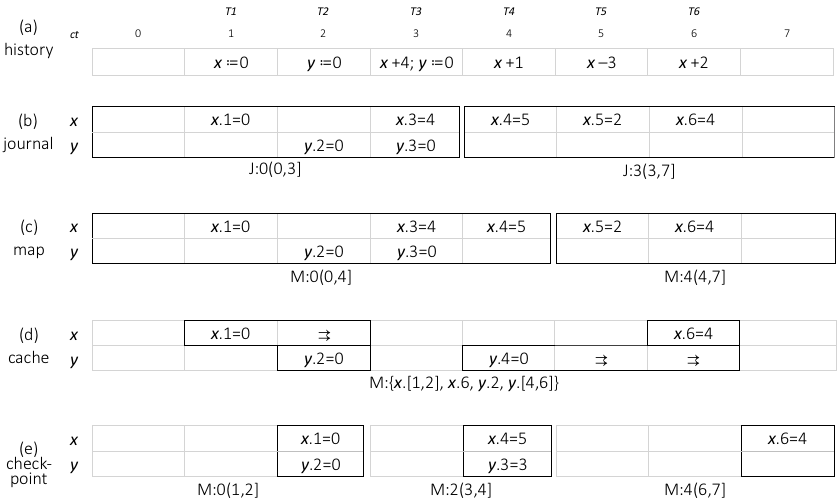
\includegraphics[width=.5\textwidth]{figures/systor-variants-and-composition.png}
  \caption[Store variants and store composition]{
    Store variants and store composition.
    % Subfigure~(a): history; the following ones different
    % variants and ranges.
    To simplify the figure, timestamps are assumed integer (scalar), and
    the history assumed sequential.
    Notation: $x,y$: keys; $\aassign{0}$: assign key with value 0;
    $+2, -3$: increment  key's value by 2, decrement by 3;
    $y.4~{+1}$: increment $y$ by 1 with commit timestamp 4.
    $\rightrightarrows$ extends validity of a cache entry; in
    \asegmentstore{J}{1}{2}{3}: J = journal{\slash}M = map,
    \lowhistory{}=1, domain $(\lowlookup{}=2, \highlookup{}=3]$.
}
  \label{fig:variants-and-composition}
\end{figure}

\section{Basic variants}
\label{sec:basic}

\subsection{Map store semantics}
\label{sec:map-store-variant}

Our first variant is the random-access \emph{map-based store}, located
either in memory or on disk.
As illustrated informally in
Figure~\ref{fig:variants-and-composition}(b), a map store can be abstracted
as an infinite matrix, with a row per key and a column per time unit.%
%
\footnote{
  % 
  In the figure, ignore for now the dividing line between 4 and 5, and
  the bound indications underneath.
  To simplify the illustration, it assumes that time ranges over the
  natural integers.
  We will consider bounding the store's size later in this paper
  (Section~\ref{sec:conductor}).
}
%
An empty store contains all \bottom{}.
The cell at index $(\akey,\atmstp)$ is populated iff some transaction
committed an update to key \akey{} at timestamp \atmstp{}.
A version remains valid until the next following version in the same
\akey{} row.
% Conversely, if key-timestamp pair $(\akey, \atmstp) \neq \bottom$, noted
% $(\akey, \atmstp) \in \dom{\astore}$, that means that a transaction with
% commit timestamp $\atmstp$ assigned $\akey$ with value $\astore(\akey,
% \atmstp)$.
% Looking up key \akey{} under snapshot timestamp \asnpsht{} returns the
% most recent version in the store whose timestamp is strictly less than
% \asnpsht{}.

The map-store algorithm is described by the semantics of
Figure~\ref{fig:map-store-semantics}.
Starting from an initially empty map store:
\begin{compactitem}
\item 
  Command \cmdLookup{\astore}{\akey}{\asnpsht} (called in the context of
  rule \initkeyrule{}), finds in store \astore{} the most recent version
  of key \akey{} that is visible from the current transaction's dependency
  timestamp \asnpsht{}.
  If there are multiple concurrent most-recent versions, it merges them.
\item
  Command \doUpdate is a no-op for this
  variant.
\item
  When a transaction commits with timestamp \acomstp{}, \doCommit{}
  eagerly copies its update to every dirty key \akey{}, from the state
  buffer into coordinates $(\akey, \acomstp)$ of the matrix.
% Removed for systor for simplicity
% %
% \footnote{
% %
%   Strictly speaking, copying only the dirty keys is not logically
%   necessary.
%   However, this is justified in practice, since the space of keys is
%   essentially unbounded (e.g., if keys are arbitrary strings).
% }
% %
\end{compactitem}

\subsection{Map store implementation}
\label{sec:map-based}

As above, we implement the map store in Java verbatim.
We purposely avoid optimisations that would obscure the intent.
We check every premise of the spec with an assertion in the Java code.
The in-memory implementation uses a standard concurrent Java hashmap to
map keys to an ordered list of timestamped versions.
Our persistent map store is the same, with the addition of Java
serialisation{\slash}deserialisation to{\slash}from disk.

As described in Figure~\ref{fig:map-store-semantics}, a lookup in the
map store queries the map with arguments \akey{} and \asnpsht{}; the map
returns the entry for $\akey$ with the highest timestamp strictly
less than \asnpsht{}.
The \doUpdate{} function is a no-op.
The \doCommit{} function adds a new version to each dirty key, with the
transaction's commit timestamp \acomstp{}; since commit timestamps are
unique, different transactions are guaranteed to write to different
locations.

This implementation assumes graceful shutdown, purposely avoiding
any complex fault-tolerance mechanism.
(We discuss fault tolerance later \commentaire[TODO]{ref?}).
More precisely, the in-memory map is assumed lost on
restart.
% The on-disk implementation assumes that before a clean power-down, in-progress
% writes first terminate.
Writing to disk is assumed idempotent: writing the same data to disk
twice (possibly with a crash in the middle) is indistinguishable from a
single write.
In case of a crash, an in-progress write may be persisted or not,
non-deterministically.

After writing the dirty keys, the \doCommit{} of the on-disk map records
the commit timestamp to one of two on-disk locations, alternating
between the two; we assume that such a write is atomic.
Each location is monotonically increasing.%
%
\footnote{
%
  Recall from Section~\ref{sec:enforce-visibility} that the coordinator
  ensures that transactions commit in growing timestamp order and that
  commit becomes visible after \doCommit{} returns.
}
%
When the store restarts after a power-down, it takes the highest of the
two, ensuring that commits are taken into account correctly.

\subsection{Journal store semantics}

Our second variant is the journal-based store.
% A journal stores computations
A journal is accessed sequentially, and materialises values lazily on
\lookup{}.%
%
\footnote{
%
  Technically, this is a redo log.
  An undo log would store inverse effects.
}
%
Figure~\ref{fig:variants-and-composition}(b) provides an informal
illustration.%
%
\footnote{
%
  Again, ignore for now the dividing line between 3 and 4, and the
  bounds indicated underneath.
}

Figure~\ref{fig:journal-store-semantics} gives the formal semantics of a
journal store.
% , represented by meta-variable \ajournal{} (in place of
% \astore{}).
Function \doUpdate{} appends an \cmdUpdateTag{} record to the journal,
containing arguments transaction identifier \atrans{}, key \akey{}, and
effect \aeffect{}.
Similarly, \doCommit{} %, called in the context of Rule \commitrule{},
appends a \jrnlCommitTag{} record containing the transaction identifier
and commit timestamp.
The read-set, dirty-set and state buffer are discarded.

The real action is in \lookup{}.
To find the value of \akey{}, it extracts from the log the effects of
all transactions that the current transaction depends upon, i.e., those
whose commit-timestamp is before \asnpsht{}, and composes these effects
(in visibility order, ignoring all but the most recent assignment, and
merging concurrent effects).

\subsection{Journal store implementation}
\label{sec:journal-implementation}

We provide an in-memory and an on-disk implementation.
We make the following assumptions of the disk.
Writes are sequentially ordered; if a write succeeds, all preceding
writes have succeeded.
There is a blocking \emph{flush} operation; if it returns successfully,
or is followed by a power-down, all preceding writes have succeeded.
If a crash occurs before \emph{flush} returns, it is guaranteed that
some prefix of the preceding writes terminated successfully.

Thus, flushing the single \jrnlCommitTag{} record to secondary storage
ensures crash-atomicity.
In the event of a crash, either the commit record and all
preceding records were written, making the whole transaction durable, or
it has not, and the transaction is aborted on recovery.

Being sequential, a persistent journal generally has better write and
worse read response time than a persistent map store.
% Our experiments in Section~\ref{sec:experiments} confirm these
% well-known differences.

Our implementation of the journal store is a straightforward,
translation of the specification into Java, deliberately avoiding
optimisations, and checking premises with assertions.
The in-memory implementation is an append-only data structure,
containing a sequence of records; the on-disk journal writes its records
to a sequential file.
There are three main types of records:
\begin{compactitem}
\item
  A \jrnlBeginTag{} record marks the beginning of a
  transaction.
  It contains its identifier and a dependency timestamp.
\item
  An \jrnlUpdateTag{} record contains an update, tagged by the
  identifier of the corresponding transaction.
\item
  A record marking the end of a transaction is either \jrnlAbortTag{}
  or \jrnlCommitTag{}.
  Both carry the transaction identifier; a \jrnlCommitTag{} also
  contains its commit timestamp \acomstp.
\end{compactitem}
Records of type \jrnlBeginTag{} and \jrnlAbortTag{} are not strictly required
by the specification, but they facilitate parsing the journal and
recovery.
\commentaire[Marc]{Add 'doBegin' to \starttxnrule{} in order to write
  the begin record.}

Disk writes are asynchronous.
However, \doCommit{} performs \emph{flush} to ensure that all the
records of the transaction are stored persistently in case of a crash.
The coordinator calls into the timestamp server to advance
$\minallowedct{}$ only once \doCommit{} has returned, after flush has
succeeded.
This ensures that the transaction becomes visible only once its commit
has persisted to disk, ensuring correct recovery after a crash.

Function $\lookup$ reads the journal sequentially, and applies the
effects of the committed transactions that are visible to the current
transaction.
When it reads an \jrnlUpdateTag{}, it defers applying it until it
reads a matching \jrnlCommitTag{} record.

The journal store writer is implemented using a single-thread executor,
to ensure that the journal is written sequentially.
Reading while a concurrent transaction is writing is not
a problem, since the timestamp server ensures that commits become visible
in increasing timestamp order.
As the journal contains all updates, the store can materialise any
version required, without any concurrency issues.

The records from multiple transactions may be mixed in the journal (they
are not necessarily in sequence).
The implementation enforces the invariant that each transaction is
structured as a \jrnlBeginTag{} record, followed by any number of
matching \jrnlUpdateTag{} records, followed either by a matching
\jrnlCommitTag{}, or a matching \jrnlAbortTag{} record.
Duplicate \jrnlCommitTag{} or \jrnlAbortTag{} records are ignored.
After a crash, the recovery procedure closes any incomplete transaction
with an \jrnlAbortTag{} record, and initialises the timestamp server with
the highest commit timestamp found in the journal.

\begin{figure}[tp]\small\centering
  % -*-mode: latex; coding: utf-8-unix -*-

\[
  \begin{array}{rcl}
    \cmdLookup{\astore}{\akey}{\asnpsht}
    & = &
      \begin{cases}
        \text{as in Fig.~\ref{fig:map-store-semantics} or~\ref{fig:journal-store-semantics}}
             & \text{if}\ (\akey, \atmstp) \in \adomain[\astore] \\
        \bottom & \text{otherwise} \\
      \end{cases}
    \\
    % 
    \cmdDoUpdate{\astore}{\atrans}{\akey}{\aeffect}
    & = & 
      \begin{cases}
        \text{as in Fig.~\ref{fig:map-store-semantics} or~\ref{fig:journal-store-semantics}}
             & \text{if}\ (\akey, \atmstp) \in \adomain[\astore] \\
        \astore & \text{otherwise} \\
      \end{cases}
    \\
    %
    \cmdDoCommit{\astore}{\atrans}{\areadset}{\adirtyset}{\astatebuf}{\acomstp}
    & = & 
      \begin{cases}
        \text{as in Fig.~\ref{fig:map-store-semantics} or~\ref{fig:journal-store-semantics}}
             & \text{if}\ (\akey, \atmstp) \in \adomain[\astore] \\
        \astore & \text{otherwise} \\
      \end{cases}
    \\
  \end{array}
\]


%% Local Variables:
%% mode: latex
%% coding: utf-8
%% ispell-local-dictionary: "en_GB"
%% mode: flyspell
%% TeX-master: "../main.tex" 
%% my-latex-bibfile: "~/svnbackup/bib/shapiro-bib-ext.bib"
%% End:

  \caption{Store \astore{} with domain
    \adomain[\astore]
  }
  \label{fig:domain-semantics}
\end{figure}
\begin{figure}[tp]
  \small\centering
    \newcommand{\OCL}[1]{\multicolumn{1}{l}{\ensuremath{#1 =}}}
  \newcommand{\OCR}[1]{\multicolumn{1}{r}{\ensuremath{#1}}}
\begin{tabular}[t]{@{}p{\columnwidth}@{}}
\OCL{\cmdLookup{\{\astore[1], \astore[2] \}}{\akey}{\asnpsht}}\\
\OCR{\max_{<} \{ \cmdLookup{\astore[1]}{\akey}{\asnpsht}, \cmdLookup{\astore[2]}{\akey}{\asnpsht} \}} \\
\OCL{\cmdDoUpdate{\{\astore[1], \astore[2] \}}{\atrans}{\akey}{\aeffect}}\\
\OCR{\cmdDoUpdate{\astore[1]}{\atrans}{\akey}{\aeffect} \parallel{} \cmdDoUpdate{\astore[2]}{\atrans}{\akey}{\aeffect}} \\
\OCL{\cmdDoCommit{\{\astore[1], \astore[2] \}}{\atrans}{\areadset}{\adirtyset}{\astatebuf}{\acomstp}} \\
\OCR{\cmdDoCommit{\astore[1]}{\atrans}{\areadset}{\adirtyset}{\astatebuf}{\acomstp} \parallel{} \cmdDoCommit{\astore[2]}{\atrans}{\areadset}{\adirtyset}{\astatebuf}{\acomstp}} \\
\end{tabular}

%% Local Variables:
%% mode: latex
%% coding: utf-8
%% ispell-local-dictionary: "en_GB"
%% mode: flyspell
%% TeX-master: "main" 
%% my-latex-bibfile: "~/svnbackup/bib/shapiro-bib-ext.bib"
%% End:

  \caption{Operations of composed store}
  \label{fig:composed-ops}
\end{figure}
\begin{figure}[tp]\small\centering
  % -*-mode: latex; coding: utf-8-unix -*-

    \[
    \inferrule[\addminirule]
    {
      \astore = \{ \astore[1], \astore[2], \ldots{} \}
      \adomain[\astore] = \adomain[{\astore[1]}] \union \adomain[{\astore[2]}] \union \ldots{}
      \forall (\akey,\atmstp) \in \adomain[{\astore[0]}] \intersect
      \adomain[\astore]:
      \cmdLookup{\astore[0]}{\akey}{\atmstp} = \cmdLookup{\astore}{\akey}{\atmstp}
      \astore' = \astore \union \astore[0]
      \adomain[\astore'] = \adomain[\astore] \union \adomain[{\astore[0]}]
    }
    {\astate
      \xrightarrow[]{\cmdAddMini{\astore}{\afield[\astore]}{\astore[0]}{\afield[{\astore[0]}]}}
      \bstate{\afield[\astore']}{\atrseta}{\atrsetc}{\atrsetr}
    }
  \]

  \[
    \inferrule[\rmvminirule]
     {
      \astore = \{ \astore[0], \astore[1], \astore[2], \ldots{} \}
      \\
      \adomain[\astore] = \adomain[{\astore[0]}] \union \adomain[{\astore[1]}] \union \adomain[{\astore[2]}] \union \ldots{}
      \\
      \astore' = \astore \setminus \astore[0]
      \\
      \adomain[\astore'] = \adomain[{\astore[1]}] \union \adomain[{\astore[2]}] \union \ldots{}
    }
    {\astate
      \xrightarrow[]{\cmdRmvMini{\astore}{\afield[\astore]}{\astore[0]}{\afield[{\astore[0]}]}}
      \bstate{\afield[\astore']}{\atrseta}{\atrsetc}{\atrsetr}
    }
  \]


%% Local Variables:
%% mode: latex
%% coding: utf-8
%% ispell-local-dictionary: "en_GB"
%% mode: flyspell
%% TeX-master: "main" 
%% my-latex-bibfile: "~/svnbackup/bib/shapiro-bib-ext.bib"
%% End:

  \caption{Operational semantics of store composition.
    \small
    \astore{} is the composition of ministores \astore[1], \astore[2],
    \ldots{}.
    \adomain[\astore] is the domain component of \afield[\astore].
  }
  \label{fig:store-composition-semantics}
\end{figure}

\section{Composing stores}
\label{sec:composed-store-variant}

The basic store variants of the previous section are
simple but have performance issues, e.g., they grow unbounded.
Modern stores improve performance with features such as caching,
write-ahead logging, layered storage, etc.
We argue in this section that these features can be represented as
\emph{composition} of our basic variants.

The composition rules are particularly simple.
A composed store is simply a set of stores (called ministores),
each restricted to a specific \emph{domain}.
The \lookup{}, \doUpdate{} and \doCommit{} operations over the
composition extend recursively to its component ministores, as
formalised in Figure~\ref{fig:composed-ops}.

For instance, a cache is an in-memory record of recently-used versions;
ignoring the details of the caching policy, the cache is a map
ministore, whose domain is an arbitrary subset of key-timestamp pairs.
For instance, Figure~\ref{fig:variants-and-composition}(d) represents a
cache containing versions $\{ (x,1), (x,6), (y,2), (y,4) \}$, where $(x,
1)$ and $(y, 4)$ are known to remain valid until timestamps 2 and 6
respectively.
A cache is fast, but must be composed with a (possibly slower)
persistent store covering the full range of keys and timestamps; for
instance either the journal in
Figure~\ref{fig:variants-and-composition}(b) or the map in~(c).

Another example is a write-ahead log (WAL).
A WAL combines a sequential, fault-tolerant journal ministore, with a
random-access map ministore.
When an update commits, it is written (in a crash-tolerant manner) to
the journal; later, it is copied and persisted to the map.
Thus, the journal's time domain includes the most recent updates,
whereas the map's is slightly delayed.
For instance, the first map in
Figure~\ref{fig:variants-and-composition}(c) might be combined with the
second journal in Subfigure~(b).
Furthermore, this WAL might be composed with the in-memory cache of
Subfigure~(d) to decrease average response time.

The LSM-Tree approach \cite{app:1730} decomposes a store into a series
of layers.
The top layer contains the most recent updates, which percolate
downwards towards the bottom layer as they age.
When reading, the system queries the layers from top to bottom in
succession, returning the first value found.
We represent this as a composition of map ministores that differ in the
time domain.

In future work, we plan to formalise sharding and geo-replication
\cite{rep:pro:sh182} by composition.

\subsection{Field and domain of a store}
\label{sec:domain}

We associate store \astore{} with auxiliary information, its
\emph{field} \afield[\astore{}].
The field is itself composed of a lower bound $\lowhistory{} \in
\Timestamptype$ and a \emph{domain} $\adomain[\astore] \subseteq {\Keytype
  \times \Timestamptype}$.
We modify the store operations \lookup{}, \doUpdate{} and \doCommit{}
to be significant only within the associated domain; outside, they are
no-ops.
This is formalised in Figure~\ref{fig:domain-semantics}.

We will call \emph{total} store one whose field is the full
universe $(0, \Keytype \times \Timestamptype)$, and
\emph{ministore} one whose domain is a strict subset.
A ministore may restrict the key domain, the time domain, or both.
For instance, \emph{sharding} composes ministores covering disjoint
subsets of the key domain.

Caches aside, the rest of this paper focuses on stores whose time domain
is a continuous \emph{segment} of time $(\lowlookup{}, \highlookup{}]$.
Timestamp \lowhistory{} is significant only for segment domains, and
represents the beginning of the history used in computing this segment.
We summarise this information with notation
\asegmentstore{X}{\lowhistory{}}{\lowlookup{}}{\highlookup{}}, where X
is M (for a map) or J (for a journal).

A \emph{checkpoint} is a map whose domain is restricted to a single
point: $(\highlookup-1, \highlookup] = \{ \highlookup \}$.
A checkpoint contains only the latest version of
each key in the range $(\lowhistory, \highlookup]$.

For instance (assuming for simplicity that timestamps are integers), a
ministore \astore{}=\asegmentstore{J}{10}{20}{30} is a journal,
representing the history between times 10 (exclusive) and 30
(inclusive), but for which $\cmdLookup{\astore}{\akey}{\atmstp}$ is
significant only if $20 < \atmstp \le 30$.
% To remain correct, it must be composed with a ministore whose history
% starts at 0, e.g., with checkpoint $[0, 9, 9]$.
Figure~\ref{fig:variants-and-composition}(b) represents two journal
ministores \asegmentstore{J}{0}{0}{3} and \asegmentstore{J}{3}{3}{7};
the second contains only the incremental effects in range $(3,7]$,
ignoring those at or before its $\lowhistory{}=3$.
Subfigure~(c) represents two map ministores; the second one reflects
only the incremental versions created starting at timestamp 5.
Subfigure~(e) shows three incremental checkpoints, recording only
the last value in the domain, and only if updated between \lowhistory{}
and \highlookup{}.

Obviously, $\lowhistory{} \le \lowlookup{} < \highlookup{}$.
Typically, either $\lowhistory{} = \lowlookup{}{}$ (it records all
versions in range) or $\lowlookup{}+1 = \highlookup{}$ (a checkpoint
summarising the updates between \lowhistory{} and \highlookup{}).

\subsection{Composition of stores}
\label{sec:store-composition}

A composed store is simply a set of ministores.
Its domain is the union of components' domains.
An operation on the composed store just calls itself recursively on the
component ministores.

Formally, consider ministores \astore[1] and \astore[2], with domains
\adomain[1] and \adomain[2] respectively.
Their composition $\{ \astore[1], \astore[2] \}$ has domain $\adomain[1]
\union \adomain[2]$.
Its operations are defined by the equations in
Figure~\ref{fig:composed-ops}, where $\parallel$ denotes parallel
composition.
%  \commentaire[TODO]{TODO}
% %
% \footnote{
%   % 
%   We defer the discussion of how to ensure the composition remains atomic
%   to Section~\ref{sec:composed-store-remains-atomic-TODO????}.
% }
% %

We showed earlier that stores are functional and that \lookup{} on any
map or journal returns the same result.
It follows that, if a key-timestamp pair is in domain of two components,
it is equivalent to perform \lookup{} on one, on the other, or on both.
Therefore it is often most efficient to perform \lookup{} on the most
recent ministore first, and to stop as soon as a \lookup{} returns an
Assignment.
Similarly, an operation can skip recursing into a component for which
the arguments are not in domain.
% Formally, $(\akey, \atmstp) \in \adomain[1] \intersect \adomain[2]
% \implies \cmdLookup{\astore[1]}{\akey}{\atmstp} =
% \cmdLookup{\astore[2]}{\akey}{\atmstp}$.
% \commentaire[TODO]{Check this assertion!  It might be incorrect for a
%   journal whose history does not start at 0.}
By abuse of notation, we identify a composed store with a store, and
note $\astore = \{ \astore[1], \astore[2] \}$.

The composition of segment stores, whose domains are adjacent or
overlap, behaves like single union segment.
For instance, in Figure~\ref{fig:variants-and-composition} the
composition of mini-journals \asegmentstore{J}{0}{0}{3} and
\asegmentstore{J}{3}{3}{7} behaves like \asegmentstore{J}{0}{0}{7}.
Similarly, combining the second checkpoint \asegmentstore{M}{2}{3}{4} with mini-map
\asegmentstore{M}{4}{4}{7} behaves like \asegmentstore{M}{2}{3}{7}.
Mini-map \asegmentstore{M}{0}{0}{4} combined with
mini-journal \asegmentstore{J}{3}{3}{7} behaves like
\asegmentstore{M}{0}{0}{7}.
In contrast, it is not useful to compose checkpoint
\asegmentstore{M}{0}{1}{2} with \asegmentstore{J}{3}{3}{7}, as this
would leave a gap.

Formally,%
%
\footnote{
  % 
  For brevity, for the rest of this section, we will use
  the abbreviations \LH{}, \LL{} and \HL{} for \lowhistory{}, \lowlookup{}
  and \highlookup{} respectively.
}
%
composing
$\asegmentstore{M}{\LH_{1}}{\LL_{1}}{\HL_{1}}$
with
$\asegmentstore{M}{\LH_{2}}{\LL_{2}}{\HL_{2}}$
where there are no \emph{gaps} between the two, i.e., $\HL_{1}
\ge \LL_{2} \land \HL_{1} \ge \LH_{2}$, behaves
like
\asegmentstore{M}{\LH_{1}}{\LL_{1}}{\HL_{2}}.
Similarly for J-segment ministores.

Another interesting case is when their histories are adjacent but not
their domains.
In this case, the history of the composition is the composition of
histories, but the domain is just the higher one.
For instance, in Figure~\ref{fig:variants-and-composition}, composing
\asegmentstore{M}{0}{0}{4} with checkpoint \asegmentstore{M}{4}{6}{7}
behaves like \asegmentstore{M}{0}{6}{7}.

Formally, if $\HL_{1} \not\ge \LL_{2} \land \HL_{1} \ge
\LH_{2}$, then the composition of
$\asegmentstore{M}{\LH_{1}}{\LL_{1}}{\HL_{1}}$ with
$\asegmentstore{M}{\LH_{2}}{\LL_{2}}{\HL_{2}}$ behaves like
\asegmentstore{M}{\LH_{1}}{\LL_{2}}{\HL_{2}}.

\subsection{Modifying a composition}
\label{sec:modify-composition}

A composition typically does not remain static but gets modified over
time.
Consider for instance the WAL, where an update is first written to a
journal, and later copied to a map.
The map's \highlookup{} is always a bit behind the most
recent commits, but increases monotonically with time.
Conversely, once an update has been copied, it can be truncated away
from the journal, increasing the latter's \lowlookup{}.
Thus a WAL is a store composed of a map and a journal, whose domains get
modified concurrently with the execution of transactions.

Figure~\ref{fig:store-composition-semantics} specifies the rules for
adding or removing a ministore.
The composed store is denoted \astore{}, with domain \adomain[\astore],
and the added{\slash}removed ministore is noted \astore[0] with domain
\adomain[{\astore[0]}].

Recall that, for any query \cmdLookup{\astore{}}{\akey{}}{\atmstp{}},
any store \astore{} that is produced by applying the transaction semantics
(Figure~\ref{fig:transaction-semantics}) returns the same result, as
long as the arguments are in domain, i.e., $(\akey, \atmstp) \in
\adomain[\astore]$.
We must ensure that this remains true for a store produced by the new
rules of Figure~\ref{fig:store-composition-semantics}.
Hence, in Rule \addminirule{}, the precondition $\forall (\akey,\atmstp)
\in \adomain[{\astore[0]}] \intersect \adomain[\astore]:
\cmdLookup{\astore[0]}{\akey}{\atmstp} =
\cmdLookup{\astore}{\akey}{\atmstp}$.

Otherwise, the rules are very simple.
\addminirule{} states that adding a ministore to a composition extends
its domain, whereas \rmvminirule{} states the reverse.

Note that there is no rule for extending or shrinking ministore's
domain, as this can be expressed as a combination of adding and
removing.
For instance, consider a composed store with a single component,
$\astore = \{ \astore[1] \}$.
For the sake of argument, say
$\astore[1]=\asegmentstore{J}{10}{20}{30}$, and we wish to extend the
store's upper bound to 45.
For this, copy the contents of \astore[1] into
$\astore[2]=\asegmentstore{J}{10}{20}{45}$; add \astore[2] to \astore{};
and finally remove \astore[1] from \astore{}.
Doing it in this order ensures that \astore{} continues to service
\lookup{}, \doUpdate{} and \doCommit{} operations correctly and without
interruption.

Let us return to the WAL, moving updates from the journal to the map and
truncating the journal.
For the sake of argument, consider a WAL
$\astore = \{
\asegmentstore{M}{0}{0}{100},
\asegmentstore{J}{100}{100}{140} \}$.
This composition has no gaps.
To represent growing the map, we add a new map
\asegmentstore{M'}{0}{0}{120}, initialised by copying the contents of
$M$, adding the result of \cmdLookup{\astore{}}{\akey{}}{\atmstp{}} for
all $\atmstp \in (100,120]$.
Once this is done, $M$ is redundant, and we remove it from \astore{}.
Alternatively, we could add an incremental segment
\asegmentstore{M''}{100}{100}{120} and not remove $M$.

Now we can truncate the journal.
We copy $J$ into \asegmentstore{J'}{110}{110}{200}, add $J'$ to
\astore{}, and remove $J$.
As we were careful to never introduce gaps, this ordering ensures that
\astore{} continues to service transactions uninterrupted.

\subsection{Total store}
\label{sec:total}

A total store is a segment store that represents the whole history,
i.e., with $\lowhistory = 0$.
% A store that is not total is useful only for partial results, and
% must be composed with one or more others.
To capture this, we add to the rules of
Figure~\ref{fig:store-composition-semantics} the following for a total
store:
\begin{inparaitem}
\item
  A total store is created as a segment store with
  $\lowhistory{}=0$.
\item
  In \rmvminirule{}, the result domain \adomain[\astore'] must be a
  segment store that satisfies $\lowhistory{}=0$.
\end{inparaitem}

Removing a ministore from the total store should not interfere with the
reads of a running transaction.
Therefore, in Figure~\ref{fig:transaction-semantics}, we add the
following premise to \commitrule{} for a total store:
$\astore.\lowlookup < \asnpsht$.
\commentaire[Marc]{We could move this premise to \initkeyrule{}; finer
  grain but possibly harder to prove.}

\commentaire[TODO]{Exhibit new total remove-ministore rule and commit rule.}

\subsection{Garbage collection}
\label{sec:gc}

As a store accumulates versions, the older versions of a key become
obsolete and take up space unnecessarily.
Garbage collection refers to the removal of such obsolete versions from
a total store.
Obviously, a removed version cannot be read by transactions any more.
Garbage collection is a direct application of store composition.
As an example, consider a store with upper bound 200; say it contains
the single segment \asegmentstore{M}{0}{0}{200}.
To garbage-collect to timestamp 100, we may replace that single segment
with the combination of a checkpoint \asegmentstore{M'}{0}{100}{100}
with incremental map \asegmentstore{M''}{0}{100}{200}.

\section{Implementing a write-ahead log by composition}
\label{sec:conductor}

To manage composition, we introduce a ``conductor'' store.%
%
\footnote{
%
  Unfortunately mixing musical metaphors.
}
%
In order to compose dynamically, the conductor supports the \addmini{},
\rmvmini{} interface of Figure~\ref{fig:store-composition-semantics}.
Although the semantics treat all ministores equally, in practice a
conductor maintains a topology of ministores and their domains, in order
\begin{inparaenum}
\item
  to access the ministores in an efficient order, and
\item
  to ensure fault tolerance.
\end{inparaenum}
As any store, the conductor also supports the \lookup{}, \doUpdate{},
\doCommit{} interface, which recurse through the ministores as specified
in Figure~\ref{fig:composed-ops}, but follows the topology.

The preferred topology (ignoring caches) has a journal at the top layer,
to leverage its write throughput and fault tolerance
properties.
Function \doCommit{} returns as soon as the journal's \doCommit{}
returns.
More details hereafter.

For performance, the conductor recurses into a ministore only if the
arguments are in its domain.
It directs \lookup{} to the top layer, then to lower ones, returning to
the client as soon as a ministore returns non-\bottom{}.
Function \doUpdate{} applies to all ministores in range, but this
generally reduces to the top-layer journal.

\subsection{Write-ahead log (WAL)}
\label{sec:WAL}

As an illustrative example, consider the case of a write-ahead log
(WAL).
% , the ``poster child'' of composition, used as a total store.

A WAL combines a journal $J$ at the top layer, with a checkpoint $M$.
An update goes first to the journal, and is later merged into the
checkpoint.
As upper bound $M.\HL{}$ of the checkpoint advances, the journal can
be truncated, advancing its lower bound $J.\LL$.
To maintain the gap-freedom invariant $J.\LL \leqq M.\HL{}$, the
correct order is therefore to first checkpoint, then truncate.

In more detail, the algorithm is as follows.
Assume the conductor is managing a total store composed of checkpoint
\asegmentstore{M}{0}{\HL-1}{\HL{}} and
\asegmentstore{J}{\LL{}}{\LL{}}{\HL{}}, where $M.\HL \geqq J.\LL$.
It creates a new checkpoint \asegmentstore{M'}{0}{\HL'-1}{\HL'{}} with
$M.\HL < M'.\HL'$.

The conductor persists a description of the checkpoint in the journal
itself.
A \ensuremath{\mathsf{CheckpointBegin}} record describes an upcoming
checkpoint, and includes both values $M.\HL$ and
$M'.\HL'$.
Once $M'$ has been persisted (remember from
Section~\ref{sec:journal-implementation} that this is atomic), the
conductor identifies (if any) the first running transaction \atrans{}
within $M'$ that terminates beyond $M'$, i.e., such that
$\atrans.\asnpsht \le M'.\HL' < \atrans.\acomstp$.
The conductor appends a \ensuremath{\mathsf{CheckpointEnd}} record to
the journal, which contains the identifier of the \jrnlBeginTag{} record
of \atrans{}.
The conductor adds the new checkpoint $M'$ to the composition, then removes
the old one $M$.
Now, the \highlookup{} of the checkpoint has safely increased to
$M'.\HL'$.

However, the conductor must not truncate away the records of any ongoing
transaction, i.e., it must stop truncation before the \jrnlBeginTag{}
record of \atrans{}.
Thus it can replace $J$ with \asegmentstore{J'}{\LL'{}}{\LL'{}}{\HL{}}
where $\LL' \leqq \atrans.\asnpsht$.
Following this ordering ensures that truncation remains transparent and
crash-tolerant.

% The first implementation challenge of the ComposedStore is to ensure
% that checkpointing is done properly.
% Here is the algorithm used to perform a checkpoint:
% \begin{enumerate}
% \item
%   Choose the next checkpoint timestamp, $t_{chk\_next}$ such as
%   $t_{chk\_next} > t_{min\_store}$ and $t_{chk\_next} < \minallowedct$
%   and $t_{chk\_next} < \atrsetr.dt$
% \item 
%   Find the commit record of the last committed transaction between
%   $t_{min\_store}$ and $t_{chk\_next}$.
%   \item Write the CheckpointBegin record with $t_{chk\_prev}$ and
%     $t_{chk\_next}$.
%   \item Lookup all the versions that are visible at $t_{chk\_next}$ and
%     write them to the Checkpoint Store.
%   \item Update the higher bound of the $CheckpointStore$ to
%     $t_{chk\_next}$.
%   \item Write the CheckpointEnd record with the $record_id$ that marks
%     the new start of the $JStore$.
%   \item Advance the lower bound of the $JStore$ to $t_{chk\_next}$.
% \end{enumerate}

% Recovery must be idempotent, ensuring that it remains safe even if it
% crashes and recovers again.
The WAL recovers as follows.
The journal recovers as in Section~\ref{sec:journal-implementation}.
If it contains a \ensuremath{\mathsf{CheckpointBegin}} record without
the matching \ensuremath{\mathsf{CheckpointEnd}} (a checkpoint might have not terminated), recovery restarts the checkpoint from the beginning using
the arguments stored in \ensuremath{\mathsf{CheckpointBegin}}; remember
that persisting a map store is idempotent.
On success, the conductor appends the missing
\ensuremath{\mathsf{CheckpointEnd}} record to the journal, and finally
re-initialises the domain of the checkpoint and the journal from the
information stored in the journal.

\begin{figure}[tp]\small\centering
  \centering
  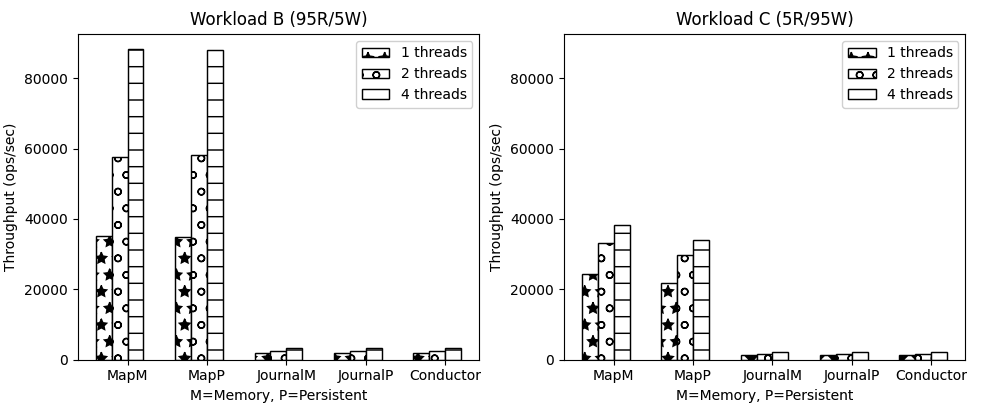
\includegraphics[width=0.5\textwidth]{figures/throughput.png}
  \caption{Average throughput of the different stores}
  \label{fig:throughput}
\end{figure}
\section{Implementation and experimental results}
\label{sec:experiments}

Our implementation code is available at
\url{https://anonymous.4open.science/r/ConductorStore-F533}.
It consists of just under 3,000 lines of Java code, containing 55
assertions.
Our experiments run on a 2021 14'' MacBook Pro under MacOS~13.2.1,
with 8 cores, 8 hardware threads, and 16\,GB of RAM and a 512\,Go SSD.
Run-time assertion checking is enabled.

\subsection{Performance comparison}

Our performance measurements are intended as an existence proof, and aim
only to show decent performance, and to compare the different variants.
We run a transactional version of YCSB, with 5 operations per
transaction, under three workloads, varying the number of reads and
writes.
Each workload executes for 60 seconds with 1, 2 or 4 concurrent
coordinator threads.

Figure~\ref{fig:throughput} plots the throughput.
The overall results are not surprising, as our implementation is
purposely not optimised.
Unexpectedly however, the on-disk map store has higher throughput than the
journal.
Indeed, as the Update rule forbids blind writes, every write is preceded
by a read, which is especially costly since a journal is sequential.
Our crash-resistant WAL implementation (marked ``Conductor'' in the
figure) suffers from the same issue.
An obvious solution will be to compose the WAL with a cache for
absorbing reads, and to allow blind writes.

\subsection{Correctness}

Assertion checking was purposely enabled (disabling it
would improve performance).
We ran YCSB up to 3 million operations on the map store,
and 200,000 operations on the journal, triggering no asserts.

\commentaire[Annette]{Unclear: ``the'' coordinator makes it sound like
  there is no concurrency.  Clarify that each store is accessed
  concurrently.}
We also validate experimentally the theoretical result that stores
are behaviourally equivalent.
To this effect, we enable the coordinator to call out to a number of
stores at the same time and to compare their return values.
This experiment runs a randomly-generated workload: the coordinator
chooses a random key, a random value and a random dependency, and a
random commit timestamp in the future; then it calls \doUpdate{} and
\doCommit{} on every store.
Truncation is disabled for this test, since it would throw away some
dependencies.
Then it reads the value back with \lookup{} and compares.
We run this experiment with an in-memory map, an in-memory journal, and
a WAL.
After 50,000 transactions, we find no divergence.